\documentclass[a4paper]{book}
\usepackage{a4wide}
\usepackage{makeidx}
\usepackage{fancyhdr}
\usepackage{graphicx}
\usepackage{multicol}
\usepackage{float}
\usepackage{textcomp}
\usepackage{alltt}
\usepackage{times}
\usepackage{ifpdf}
\ifpdf
\usepackage[pdftex,
            pagebackref=true,
            colorlinks=true,
            linkcolor=blue,
            unicode
           ]{hyperref}
\else
\usepackage[ps2pdf,
            pagebackref=true,
            colorlinks=true,
            linkcolor=blue,
            unicode
           ]{hyperref}
\usepackage{pspicture}
\fi
\usepackage[utf8]{inputenc}
\usepackage{polski}
\usepackage[T1]{fontenc}

\usepackage{doxygen}
\makeindex
\setcounter{tocdepth}{1}
\renewcommand{\footrulewidth}{0.4pt}
\begin{document}
\begin{titlepage}
\vspace*{7cm}
\begin{center}
{\Large Salvador Project \\[1ex]\large wersja 1.0 }\\
\vspace*{1cm}
{\large Wygenerowano przez Doxygen 1.5.5}\\
\vspace*{0.5cm}
{\small Sat Aug 16 12:25:33 2008}\\
\end{center}
\end{titlepage}
\clearemptydoublepage
\pagenumbering{roman}
\tableofcontents
\clearemptydoublepage
\pagenumbering{arabic}
\chapter{Indeks klas}
\section{Hierarchia klas}
Ta lista dziedziczenia posortowana jest z grubsza, choć nie całkowicie, alfabetycznie:\begin{CompactList}
\item SAbstractMachine\begin{CompactList}
\item \contentsline{section}{SDataMachine}{\pageref{classSDataMachine}}{}
\end{CompactList}
\item SAbstractPointer\begin{CompactList}
\item \contentsline{section}{SDataImagePointer}{\pageref{classSDataImagePointer}}{}
\end{CompactList}
\item \contentsline{section}{SCodeGrid}{\pageref{classSCodeGrid}}{}
\item \contentsline{section}{SDataStats}{\pageref{classSDataStats}}{}
\item \contentsline{section}{SImage}{\pageref{classSImage}}{}
\item \contentsline{section}{SVirtualMachine}{\pageref{classSVirtualMachine}}{}
\end{CompactList}

\chapter{Indeks klas}
\section{Lista klas}
Tutaj znajdują się klasy, struktury, unie i interfejsy wraz z ich krótkimi opisami:\begin{CompactList}
\item\contentsline{section}{\hyperlink{classSCodeGrid}{SCodeGrid} (Siatka kodu języka Salvador )}{\pageref{classSCodeGrid}}{}
\item\contentsline{section}{\hyperlink{classSDataImagePointer}{SDataImagePointer} (Głowica maszyny obsługująca obraz danych )}{\pageref{classSDataImagePointer}}{}
\item\contentsline{section}{\hyperlink{classSDataMachine}{SDataMachine} (Maszyna danych, obsługująca obraz danych )}{\pageref{classSDataMachine}}{}
\item\contentsline{section}{\hyperlink{classSDataStats}{SDataStats} (Informacje o działaniu maszyny danych )}{\pageref{classSDataStats}}{}
\item\contentsline{section}{\hyperlink{classSImage}{SImage} (Rozbudowa QImage o odpowiednie metody rysowania kształtów na bitmapie )}{\pageref{classSImage}}{}
\item\contentsline{section}{\hyperlink{classSVirtualMachine}{SVirtualMachine} (Wirtualna maszyna Salvadora - najbardziej \char`\"{}zewnętrzna\char`\"{} klasa całego projektu )}{\pageref{classSVirtualMachine}}{}
\end{CompactList}

\chapter{Indeks plików}
\section{Lista plików}
Tutaj znajduje się lista wszystkich udokumentowanych plików z ich krótkimi opisami:\begin{CompactList}
\item\contentsline{section}{src/\hyperlink{debug_8h}{debug.h} (Plik nagłówkowy debuggera )}{\pageref{debug_8h}}{}
\item\contentsline{section}{src/\hyperlink{test_8cpp}{test.cpp} (Plik z kodem źródłowym aplikacji )}{\pageref{test_8cpp}}{}
\item\contentsline{section}{src/core/\hyperlink{sabstractgrid_8cpp}{sabstractgrid.cpp} (Plik z kodem źródłowym klasy \hyperlink{classSAbstractGrid}{SAbstractGrid} )}{\pageref{sabstractgrid_8cpp}}{}
\item\contentsline{section}{src/core/\hyperlink{sabstractgrid_8h}{sabstractgrid.h} (Plik nagłówkowy klasy \hyperlink{classSAbstractGrid}{SAbstractGrid} )}{\pageref{sabstractgrid_8h}}{}
\item\contentsline{section}{src/core/\hyperlink{sabstractmachine_8cpp}{sabstractmachine.cpp} (Plik z kodem źródłowym klasy \hyperlink{classSAbstractMachine}{SAbstractMachine} )}{\pageref{sabstractmachine_8cpp}}{}
\item\contentsline{section}{src/core/\hyperlink{sabstractmachine_8h}{sabstractmachine.h} (Plik nagłówkowy klasy \hyperlink{classSAbstractMachine}{SAbstractMachine} )}{\pageref{sabstractmachine_8h}}{}
\item\contentsline{section}{src/core/\hyperlink{sabstractpointer_8cpp}{sabstractpointer.cpp} (Plik z kodem źródłowym klasy \hyperlink{classSAbstractPointer}{SAbstractPointer} )}{\pageref{sabstractpointer_8cpp}}{}
\item\contentsline{section}{src/core/\hyperlink{sabstractpointer_8h}{sabstractpointer.h} (Plik nagłówkowy klasy \hyperlink{classSAbstractPointer}{SAbstractPointer} )}{\pageref{sabstractpointer_8h}}{}
\item\contentsline{section}{src/core/\hyperlink{scodegrid_8cpp}{scodegrid.cpp} (Plik z kodem źródłowym klasy \hyperlink{classSCodeGrid}{SCodeGrid} )}{\pageref{scodegrid_8cpp}}{}
\item\contentsline{section}{src/core/\hyperlink{scodegrid_8h}{scodegrid.h} (Plik nagłówkowy klasy \hyperlink{classSCodeGrid}{SCodeGrid} )}{\pageref{scodegrid_8h}}{}
\item\contentsline{section}{src/core/\hyperlink{scodeimage_8h}{scodeimage.h} (Plik nagłówkowy klasy SCodeImage )}{\pageref{scodeimage_8h}}{}
\item\contentsline{section}{src/core/\hyperlink{scodeimagepointer_8cpp}{scodeimagepointer.cpp} (Plik z kodem źródłowym klasy \hyperlink{classSCodeImagePointer}{SCodeImagePointer} )}{\pageref{scodeimagepointer_8cpp}}{}
\item\contentsline{section}{src/core/\hyperlink{scodeimagepointer_8h}{scodeimagepointer.h} (Plik nagłówkowy klasy \hyperlink{classSCodeImagePointer}{SCodeImagePointer} )}{\pageref{scodeimagepointer_8h}}{}
\item\contentsline{section}{src/core/\hyperlink{scodemachine_8cpp}{scodemachine.cpp} (Plik z kodem źródłowym klasy \hyperlink{classSCodeMachine}{SCodeMachine} )}{\pageref{scodemachine_8cpp}}{}
\item\contentsline{section}{src/core/\hyperlink{scodemachine_8h}{scodemachine.h} (Plik nagłówkowy klasy \hyperlink{classSCodeMachine}{SCodeMachine} )}{\pageref{scodemachine_8h}}{}
\item\contentsline{section}{src/core/\hyperlink{sdatagrid_8cpp}{sdatagrid.cpp} (Plik z kodem źródłowym klasy \hyperlink{classSDataGrid}{SDataGrid} )}{\pageref{sdatagrid_8cpp}}{}
\item\contentsline{section}{src/core/\hyperlink{sdatagrid_8h}{sdatagrid.h} (Plik nagłówkowy klasy \hyperlink{classSDataGrid}{SDataGrid} )}{\pageref{sdatagrid_8h}}{}
\item\contentsline{section}{src/core/\hyperlink{sdataimagepointer_8cpp}{sdataimagepointer.cpp} (Plik z kodem źródłowym klasy \hyperlink{classSDataImagePointer}{SDataImagePointer} )}{\pageref{sdataimagepointer_8cpp}}{}
\item\contentsline{section}{src/core/\hyperlink{sdataimagepointer_8h}{sdataimagepointer.h} (Plik nagłówkowy klasy \hyperlink{classSDataImagePointer}{SDataImagePointer} )}{\pageref{sdataimagepointer_8h}}{}
\item\contentsline{section}{src/core/\hyperlink{sdatamachine_8cpp}{sdatamachine.cpp} (Plik z kodem źródłowym klasy \hyperlink{classSDataMachine}{SDataMachine} )}{\pageref{sdatamachine_8cpp}}{}
\item\contentsline{section}{src/core/\hyperlink{sdatamachine_8h}{sdatamachine.h} (Plik nagłówkowy klasy \hyperlink{classSDataMachine}{SDataMachine} )}{\pageref{sdatamachine_8h}}{}
\item\contentsline{section}{src/core/\hyperlink{senums_8h}{senums.h} (Wszystkie enumeracje )}{\pageref{senums_8h}}{}
\item\contentsline{section}{src/core/\hyperlink{simage_8h}{simage.h} (Plik nagłówkowy klasy \hyperlink{classSImage}{SImage} )}{\pageref{simage_8h}}{}
\item\contentsline{section}{src/core/\hyperlink{svirtualmachine_8cpp}{svirtualmachine.cpp} (Plik z kodem źródłowym klasy \hyperlink{classSVirtualMachine}{SVirtualMachine} )}{\pageref{svirtualmachine_8cpp}}{}
\item\contentsline{section}{src/core/\hyperlink{svirtualmachine_8h}{svirtualmachine.h} (Plik nagłówkowy klasy \hyperlink{classSVirtualMachine}{SVirtualMachine} )}{\pageref{svirtualmachine_8h}}{}
\end{CompactList}

\chapter{Dokumentacja klas}
\hypertarget{classSCodeGrid}{
\section{Dokumentacja klasy SCodeGrid}
\label{classSCodeGrid}\index{SCodeGrid@{SCodeGrid}}
}
siatka kodu  


{\tt \#include $<$scodegrid.h$>$}

Diagram dziedziczenia dla SCodeGrid:\begin{figure}[H]
\begin{center}
\leavevmode
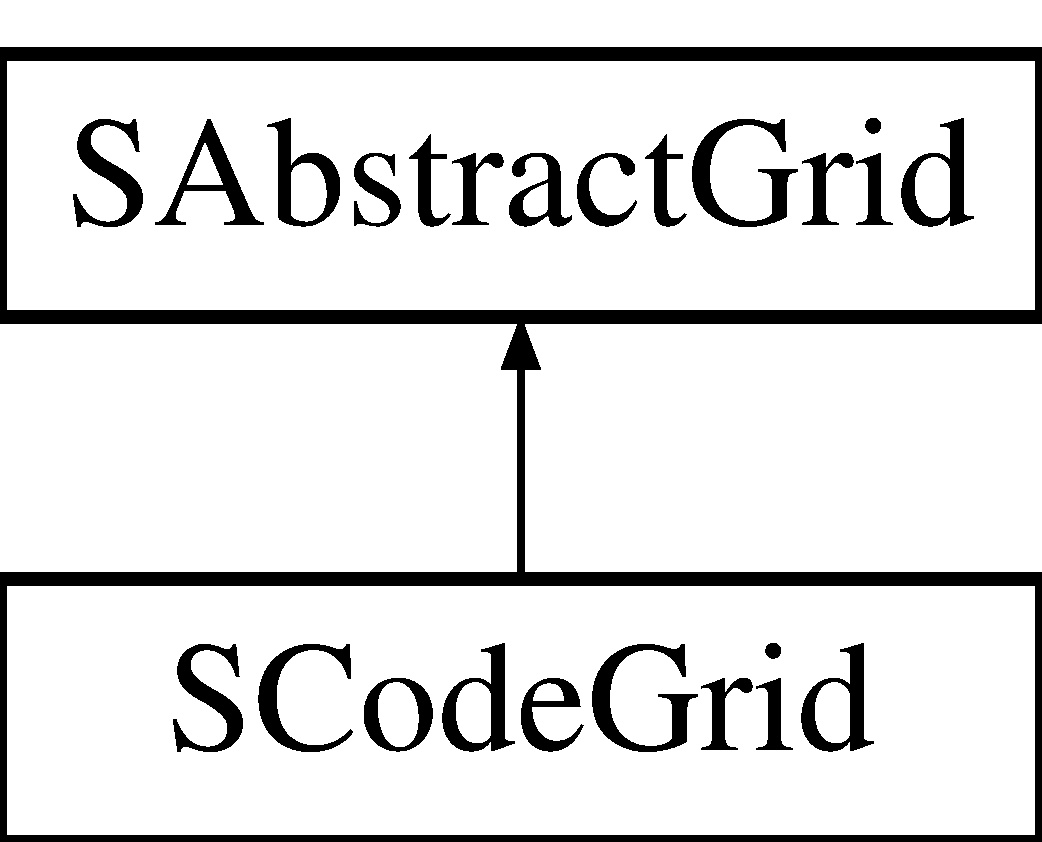
\includegraphics[height=2cm]{classSCodeGrid}
\end{center}
\end{figure}
\subsection*{Metody publiczne}
\begin{CompactItemize}
\item 
\hyperlink{classSCodeGrid_e430762ac9855cd60f8d5a57c46428b9}{SCodeGrid} (std::string, \hyperlink{senums_8h_1a2ae45552936d27425f99e1c187b043}{SCodeTypes})
\item 
\hyperlink{classSCodeGrid_c150afdd8f27785b5ddf5669a4d90332}{$\sim$SCodeGrid} ()
\item 
\hypertarget{classSCodeGrid_c57d52a49a55c91068fe0eb541e721f8}{
int \textbf{getValueAt} (int, int)}
\label{classSCodeGrid_c57d52a49a55c91068fe0eb541e721f8}

\item 
\hypertarget{classSCodeGrid_c01feeae87539b97aed07d67b975f174}{
void \textbf{\_\-\_\-dev\_\-\_\-printConsole} (int, int)}
\label{classSCodeGrid_c01feeae87539b97aed07d67b975f174}

\item 
\hypertarget{classSCodeGrid_c5754181e1266e23935d84f3beeb5979}{
int \textbf{\_\-\_\-dev\_\-\_\-transformCharToBinary} (char)}
\label{classSCodeGrid_c5754181e1266e23935d84f3beeb5979}

\item 
\hypertarget{classSCodeGrid_75d1d340ee3c5704527e793f2e71e93b}{
char \textbf{\_\-\_\-dev\_\-\_\-transformBinaryToChar} (int)}
\label{classSCodeGrid_75d1d340ee3c5704527e793f2e71e93b}

\end{CompactItemize}
\subsection*{Metody chronione}
\begin{CompactItemize}
\item 
int \hyperlink{classSCodeGrid_46ed88ad7346788efb14c40cbd836981}{readFromFile} (std::string)
\item 
\hypertarget{classSCodeGrid_f15ba156433f88a40887e5ba72d9201a}{
void \textbf{constructGrid} ()}
\label{classSCodeGrid_f15ba156433f88a40887e5ba72d9201a}

\item 
\hypertarget{classSCodeGrid_6bd4c1bf841bd09c2ffb2e019c08b4ed}{
void \textbf{destructGrid} ()}
\label{classSCodeGrid_6bd4c1bf841bd09c2ffb2e019c08b4ed}

\end{CompactItemize}
\subsection*{Atrybuty chronione}
\begin{CompactItemize}
\item 
\hypertarget{classSCodeGrid_445b4bd8cca6ddb7100afa621f5722b0}{
\hyperlink{senums_8h_b1c3fa9dccd3f8afa81e14a98d9a7d1e}{SInstructions} $\ast$$\ast$ \textbf{instruction\_\-grid}}
\label{classSCodeGrid_445b4bd8cca6ddb7100afa621f5722b0}

\end{CompactItemize}


\subsection{Opis szczegółowy}
siatka kodu 

2 cele:

\begin{itemize}
\item testowanie (development)\item nakładanie na obrazek siatki kodu (celem stworzenia obrazka zawierającego program) \end{itemize}


\subsection{Dokumentacja konstruktora i destruktora}
\hypertarget{classSCodeGrid_e430762ac9855cd60f8d5a57c46428b9}{
\index{SCodeGrid@{SCodeGrid}!SCodeGrid@{SCodeGrid}}
\index{SCodeGrid@{SCodeGrid}!SCodeGrid@{SCodeGrid}}
\subsubsection[{SCodeGrid}]{\setlength{\rightskip}{0pt plus 5cm}SCodeGrid::SCodeGrid (std::string {\em filename}, \/  {\bf SCodeTypes} {\em CODE\_\-TYPE})}}
\label{classSCodeGrid_e430762ac9855cd60f8d5a57c46428b9}


Konstruktor siatki kodu. \hypertarget{classSCodeGrid_c150afdd8f27785b5ddf5669a4d90332}{
\index{SCodeGrid@{SCodeGrid}!$\sim$SCodeGrid@{$\sim$SCodeGrid}}
\index{$\sim$SCodeGrid@{$\sim$SCodeGrid}!SCodeGrid@{SCodeGrid}}
\subsubsection[{$\sim$SCodeGrid}]{\setlength{\rightskip}{0pt plus 5cm}SCodeGrid::$\sim$SCodeGrid ()}}
\label{classSCodeGrid_c150afdd8f27785b5ddf5669a4d90332}


Destruktor siatki kodu. 

\subsection{Dokumentacja funkcji składowych}
\hypertarget{classSCodeGrid_46ed88ad7346788efb14c40cbd836981}{
\index{SCodeGrid@{SCodeGrid}!readFromFile@{readFromFile}}
\index{readFromFile@{readFromFile}!SCodeGrid@{SCodeGrid}}
\subsubsection[{readFromFile}]{\setlength{\rightskip}{0pt plus 5cm}int SCodeGrid::readFromFile (std::string {\em filename})\hspace{0.3cm}{\tt  \mbox{[}protected\mbox{]}}}}
\label{classSCodeGrid_46ed88ad7346788efb14c40cbd836981}


\begin{Desc}
\item[Zwraca:]kod błędu: 0: ok 1: nie ma takiego pliku 2: błędny format wejścia \end{Desc}


Dokumentacja dla tej klasy została wygenerowana z plików:\begin{CompactItemize}
\item 
src/core/\hyperlink{scodegrid_8h}{scodegrid.h}\item 
src/core/\hyperlink{scodegrid_8cpp}{scodegrid.cpp}\end{CompactItemize}

\hypertarget{classSDataImagePointer}{
\section{Dokumentacja klasy SDataImagePointer}
\label{classSDataImagePointer}\index{SDataImagePointer@{SDataImagePointer}}
}
głowica maszyny obsługująca obraz danych  


{\tt \#include $<$sdataimagepointer.h$>$}

Diagram dziedziczenia dla SDataImagePointer:\begin{figure}[H]
\begin{center}
\leavevmode
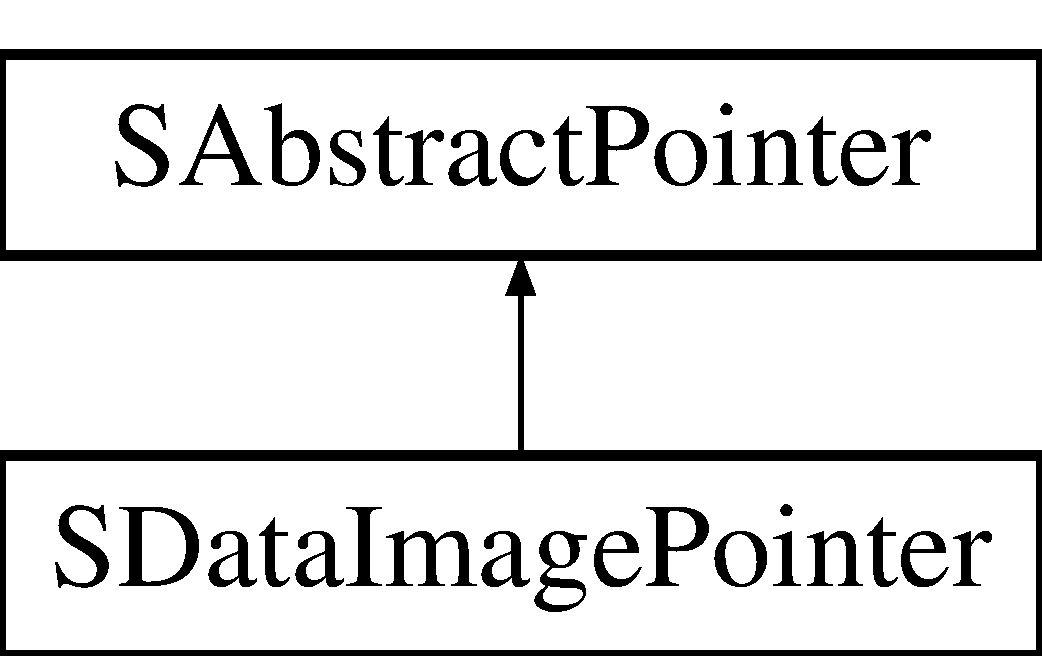
\includegraphics[height=2cm]{classSDataImagePointer}
\end{center}
\end{figure}
\subsection*{Metody publiczne}
\begin{CompactItemize}
\item 
\hyperlink{classSDataImagePointer_2ffb42e886f442004cd21617a6ea034d}{SDataImagePointer} ()
\item 
\hyperlink{classSDataImagePointer_8f96c4dc8dc25e0ff5cccb2e693ffcc8}{$\sim$SDataImagePointer} ()
\item 
int \hyperlink{classSDataImagePointer_87bb92d4bb0336b4723c64d03df9987c}{moveLeft} ()
\begin{CompactList}\small\item\em przesuwa głowicę maszyny danych w lewo \item\end{CompactList}\item 
int \hyperlink{classSDataImagePointer_9cc51881224c9e157e96d5e36189e54a}{moveRight} ()
\begin{CompactList}\small\item\em przesuwa głowicę maszyny danych w prawo \item\end{CompactList}\item 
\hypertarget{classSDataImagePointer_0cdd7239181d6f12bf6df551defaa769}{
int \textbf{increaseCellValue} ()}
\label{classSDataImagePointer_0cdd7239181d6f12bf6df551defaa769}

\item 
\hypertarget{classSDataImagePointer_0461b9855715a2d296e19865517f7f36}{
int \textbf{decreaseCellValue} ()}
\label{classSDataImagePointer_0461b9855715a2d296e19865517f7f36}

\item 
\hypertarget{classSDataImagePointer_ee071148492c43291fd01fd035f6398a}{
int \textbf{zeroCellValue} ()}
\label{classSDataImagePointer_ee071148492c43291fd01fd035f6398a}

\end{CompactItemize}


\subsection{Opis szczegółowy}
głowica maszyny obsługująca obraz danych 

Obiekt klasy \hyperlink{classSDataImagePointer}{SDataImagePointer} jest swoistym wskaźnikiem na daną komórkę obrazu danych. Maszyna danych (\hyperlink{classSDataMachine}{SDataMachine}) wykorzystuje głowicę, by dzięki niej odczytywać wartości z obrazu danych (SDataImage) oraz by na tym obrazie zapisywać nowe wartości. 

\subsection{Dokumentacja konstruktora i destruktora}
\hypertarget{classSDataImagePointer_2ffb42e886f442004cd21617a6ea034d}{
\index{SDataImagePointer@{SDataImagePointer}!SDataImagePointer@{SDataImagePointer}}
\index{SDataImagePointer@{SDataImagePointer}!SDataImagePointer@{SDataImagePointer}}
\subsubsection[{SDataImagePointer}]{\setlength{\rightskip}{0pt plus 5cm}SDataImagePointer::SDataImagePointer ()}}
\label{classSDataImagePointer_2ffb42e886f442004cd21617a6ea034d}


Konstruktor głowicy obrazu danych. Nie robi nic szczególnego. \hypertarget{classSDataImagePointer_8f96c4dc8dc25e0ff5cccb2e693ffcc8}{
\index{SDataImagePointer@{SDataImagePointer}!$\sim$SDataImagePointer@{$\sim$SDataImagePointer}}
\index{$\sim$SDataImagePointer@{$\sim$SDataImagePointer}!SDataImagePointer@{SDataImagePointer}}
\subsubsection[{$\sim$SDataImagePointer}]{\setlength{\rightskip}{0pt plus 5cm}SDataImagePointer::$\sim$SDataImagePointer ()}}
\label{classSDataImagePointer_8f96c4dc8dc25e0ff5cccb2e693ffcc8}


Destruktor głowicy obrazu danych. Nie robi nic szczególnego. 

\subsection{Dokumentacja funkcji składowych}
\hypertarget{classSDataImagePointer_87bb92d4bb0336b4723c64d03df9987c}{
\index{SDataImagePointer@{SDataImagePointer}!moveLeft@{moveLeft}}
\index{moveLeft@{moveLeft}!SDataImagePointer@{SDataImagePointer}}
\subsubsection[{moveLeft}]{\setlength{\rightskip}{0pt plus 5cm}int SDataImagePointer::moveLeft ()}}
\label{classSDataImagePointer_87bb92d4bb0336b4723c64d03df9987c}


przesuwa głowicę maszyny danych w lewo 

Najpierw ustalony jest nowy kierunek ruchu (SDirections) - w lewo, następnie głowica przesuwana jest o jedno pole (w ustalonym kierunku). Efektem przesunięcia głowicy jest zmiana jej współrzędnych względem obrazu danych. \begin{Desc}
\item[Zwraca:]? \end{Desc}
\hypertarget{classSDataImagePointer_9cc51881224c9e157e96d5e36189e54a}{
\index{SDataImagePointer@{SDataImagePointer}!moveRight@{moveRight}}
\index{moveRight@{moveRight}!SDataImagePointer@{SDataImagePointer}}
\subsubsection[{moveRight}]{\setlength{\rightskip}{0pt plus 5cm}int SDataImagePointer::moveRight ()}}
\label{classSDataImagePointer_9cc51881224c9e157e96d5e36189e54a}


przesuwa głowicę maszyny danych w prawo 

Najpierw ustalony jest nowy kierunek ruchu (SDirections) - w prawo, następnie głowica przesuwana jest o jedno pole (w ustalonym kierunku). Efektem przesunięcia głowicy jest zmiana jej współrzędnych względem obrazu danych. \begin{Desc}
\item[Zwraca:]? \end{Desc}


Dokumentacja dla tej klasy została wygenerowana z plików:\begin{CompactItemize}
\item 
src/core/\hyperlink{sdataimagepointer_8h}{sdataimagepointer.h}\item 
src/core/\hyperlink{sdataimagepointer_8cpp}{sdataimagepointer.cpp}\end{CompactItemize}

\hypertarget{classSDataMachine}{
\section{Dokumentacja klasy SDataMachine}
\label{classSDataMachine}\index{SDataMachine@{SDataMachine}}
}
maszyna danych, obsługująca obraz danych  


{\tt \#include $<$sdatamachine.h$>$}

Diagram dziedziczenia dla SDataMachine:\begin{figure}[H]
\begin{center}
\leavevmode
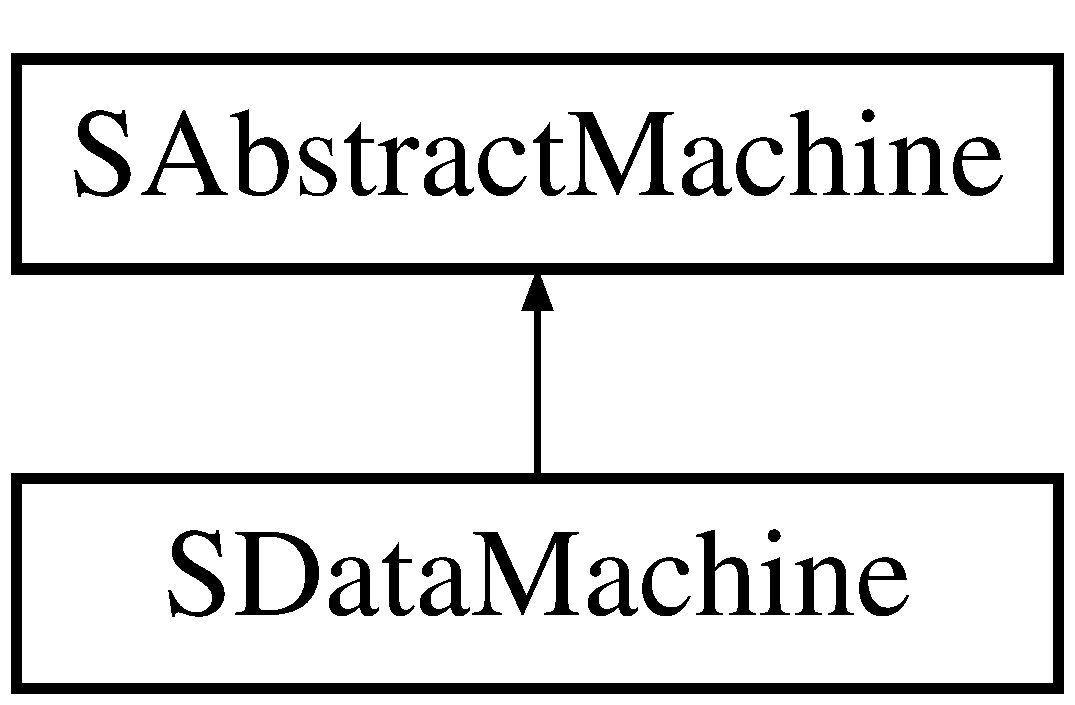
\includegraphics[height=2cm]{classSDataMachine}
\end{center}
\end{figure}
\subsection*{Metody publiczne}
\begin{CompactItemize}
\item 
\hyperlink{classSDataMachine_3d894df00bd2283c717a827e27138812}{SDataMachine} ()
\begin{CompactList}\small\item\em konstruktor \item\end{CompactList}\item 
\hyperlink{classSDataMachine_59bc85b25930729cbe3046e81f49f909}{$\sim$SDataMachine} ()
\begin{CompactList}\small\item\em destruktor \item\end{CompactList}\item 
void \hyperlink{classSDataMachine_38cc38f27606be24fc609d461d25ae2f}{setVerbosity} (bool)
\item 
bool \hyperlink{classSDataMachine_10eb8f56cf6235455a26c5c673b8fe15}{pushPointer} ()
\item 
void \hyperlink{classSDataMachine_b863ea9a42568d7555cc146ded9f2d88}{clearData} ()
\item 
int \hyperlink{classSDataMachine_3a191be9cab718274d6bd75e01cc2a26}{getPointedValue} ()
\item 
void \hyperlink{classSDataMachine_5b46d50c18bec1bcfd5232bec3875fd5}{executeTurnLeft} ()
\item 
void \hyperlink{classSDataMachine_fb6f52c7f14afa51eed848f354d57924}{executeTurnRight} ()
\item 
void \hyperlink{classSDataMachine_27c3e6dfe9ac45f9d5eed7c97f96abd8}{executeZero} ()
\item 
void \hyperlink{classSDataMachine_85832e07e2fb8ae32160fe0c95a487d2}{executeSucc} ()
\item 
void \hyperlink{classSDataMachine_87cfad868b3ea0a0e60f776ad3773678}{executePred} ()
\item 
\hypertarget{classSDataMachine_9680a908e0343de539ffd7a83d17dd11}{
void \textbf{\_\-\_\-dev\_\-\_\-initGrid} ()}
\label{classSDataMachine_9680a908e0343de539ffd7a83d17dd11}

\item 
\hypertarget{classSDataMachine_66c35c3c879c06903f306825ccaade7f}{
void \textbf{\_\-\_\-dev\_\-\_\-destroyGrid} ()}
\label{classSDataMachine_66c35c3c879c06903f306825ccaade7f}

\item 
\hypertarget{classSDataMachine_da92c5d20a64279ff191059705c3070f}{
void \textbf{\_\-\_\-dev\_\-\_\-printConsole} ()}
\label{classSDataMachine_da92c5d20a64279ff191059705c3070f}

\item 
\hypertarget{classSDataMachine_3d2383297382e73c4f61f7fc231c34b7}{
void \textbf{\_\-\_\-dev\_\-\_\-printPointer} ()}
\label{classSDataMachine_3d2383297382e73c4f61f7fc231c34b7}

\item 
\hypertarget{classSDataMachine_ec760b755d01ea8c9ef3d37aa8f749d2}{
void \textbf{\_\-\_\-dev\_\-\_\-printGrid} ()}
\label{classSDataMachine_ec760b755d01ea8c9ef3d37aa8f749d2}

\end{CompactItemize}


\subsection{Opis szczegółowy}
maszyna danych, obsługująca obraz danych 

Obiekt klasy \hyperlink{classSDataMachine}{SDataMachine} to tzw. \char`\"{}maszyna danych\char`\"{} która obsługuje dane programu wykonywanego przez Wirtualną Maszynę Salvadora. Maszyna ta posiada swój log (dziennik wszystkich wykonywanych operacji) w obiekcie klasy SDataStats oraz posiada sam obraz danych, będący graficzną reprezentacją danych wykonywanego programu. 

\subsection{Dokumentacja konstruktora i destruktora}
\hypertarget{classSDataMachine_3d894df00bd2283c717a827e27138812}{
\index{SDataMachine@{SDataMachine}!SDataMachine@{SDataMachine}}
\index{SDataMachine@{SDataMachine}!SDataMachine@{SDataMachine}}
\subsubsection[{SDataMachine}]{\setlength{\rightskip}{0pt plus 5cm}SDataMachine::SDataMachine ()}}
\label{classSDataMachine_3d894df00bd2283c717a827e27138812}


konstruktor 

Tworzy 3 obiekty, do których ma zapisane referencje:\begin{itemize}
\item log operacji maszyny danych (SDataStats)\item obraz danych (SDataImage)\item głowica maszyny danych (\hyperlink{classSDataImagePointer}{SDataImagePointer}) Maszyna danych w trakcie swojego działania będzie z nich cały czas korzystać \end{itemize}
\hypertarget{classSDataMachine_59bc85b25930729cbe3046e81f49f909}{
\index{SDataMachine@{SDataMachine}!$\sim$SDataMachine@{$\sim$SDataMachine}}
\index{$\sim$SDataMachine@{$\sim$SDataMachine}!SDataMachine@{SDataMachine}}
\subsubsection[{$\sim$SDataMachine}]{\setlength{\rightskip}{0pt plus 5cm}SDataMachine::$\sim$SDataMachine ()}}
\label{classSDataMachine_59bc85b25930729cbe3046e81f49f909}


destruktor 

Niszczy 3 obiekty, niezbędne do działania maszyny:\begin{itemize}
\item log operacji maszyny danych (SDataStats)\item obraz danych (SDataImage)\item głowica maszyny danych (\hyperlink{classSDataImagePointer}{SDataImagePointer}) \end{itemize}


\subsection{Dokumentacja funkcji składowych}
\hypertarget{classSDataMachine_b863ea9a42568d7555cc146ded9f2d88}{
\index{SDataMachine@{SDataMachine}!clearData@{clearData}}
\index{clearData@{clearData}!SDataMachine@{SDataMachine}}
\subsubsection[{clearData}]{\setlength{\rightskip}{0pt plus 5cm}void SDataMachine::clearData ()}}
\label{classSDataMachine_b863ea9a42568d7555cc146ded9f2d88}


Czyści dane przechowywane przez maszynę danych. \hypertarget{classSDataMachine_87cfad868b3ea0a0e60f776ad3773678}{
\index{SDataMachine@{SDataMachine}!executePred@{executePred}}
\index{executePred@{executePred}!SDataMachine@{SDataMachine}}
\subsubsection[{executePred}]{\setlength{\rightskip}{0pt plus 5cm}void SDataMachine::executePred ()}}
\label{classSDataMachine_87cfad868b3ea0a0e60f776ad3773678}


Wykonuje instrukcję Salvadora ZMNIEJSZ. \hypertarget{classSDataMachine_85832e07e2fb8ae32160fe0c95a487d2}{
\index{SDataMachine@{SDataMachine}!executeSucc@{executeSucc}}
\index{executeSucc@{executeSucc}!SDataMachine@{SDataMachine}}
\subsubsection[{executeSucc}]{\setlength{\rightskip}{0pt plus 5cm}void SDataMachine::executeSucc ()}}
\label{classSDataMachine_85832e07e2fb8ae32160fe0c95a487d2}


Wykonuje instrukcję Salvadora ZWIĘKSZ. \hypertarget{classSDataMachine_5b46d50c18bec1bcfd5232bec3875fd5}{
\index{SDataMachine@{SDataMachine}!executeTurnLeft@{executeTurnLeft}}
\index{executeTurnLeft@{executeTurnLeft}!SDataMachine@{SDataMachine}}
\subsubsection[{executeTurnLeft}]{\setlength{\rightskip}{0pt plus 5cm}void SDataMachine::executeTurnLeft ()}}
\label{classSDataMachine_5b46d50c18bec1bcfd5232bec3875fd5}


Wykonuje instrukcję Salvadora PRZESUŃ GŁOWICĘ DANYCH W LEWO. \hypertarget{classSDataMachine_fb6f52c7f14afa51eed848f354d57924}{
\index{SDataMachine@{SDataMachine}!executeTurnRight@{executeTurnRight}}
\index{executeTurnRight@{executeTurnRight}!SDataMachine@{SDataMachine}}
\subsubsection[{executeTurnRight}]{\setlength{\rightskip}{0pt plus 5cm}void SDataMachine::executeTurnRight ()}}
\label{classSDataMachine_fb6f52c7f14afa51eed848f354d57924}


Wykonuje instrukcję Salvadora PRZESUŃ GŁOWICĘ DANYCH W PRAWO. \hypertarget{classSDataMachine_27c3e6dfe9ac45f9d5eed7c97f96abd8}{
\index{SDataMachine@{SDataMachine}!executeZero@{executeZero}}
\index{executeZero@{executeZero}!SDataMachine@{SDataMachine}}
\subsubsection[{executeZero}]{\setlength{\rightskip}{0pt plus 5cm}void SDataMachine::executeZero ()}}
\label{classSDataMachine_27c3e6dfe9ac45f9d5eed7c97f96abd8}


Wykonuje instrukcję Salvadora ZERUJ. \hypertarget{classSDataMachine_3a191be9cab718274d6bd75e01cc2a26}{
\index{SDataMachine@{SDataMachine}!getPointedValue@{getPointedValue}}
\index{getPointedValue@{getPointedValue}!SDataMachine@{SDataMachine}}
\subsubsection[{getPointedValue}]{\setlength{\rightskip}{0pt plus 5cm}int SDataMachine::getPointedValue ()}}
\label{classSDataMachine_3a191be9cab718274d6bd75e01cc2a26}


Zwraca wartość wskazywaną przez głowicę danych na obrazie danych. \begin{Desc}
\item[Zwraca:]wartość wskazywana przez głowicę \end{Desc}
\hypertarget{classSDataMachine_10eb8f56cf6235455a26c5c673b8fe15}{
\index{SDataMachine@{SDataMachine}!pushPointer@{pushPointer}}
\index{pushPointer@{pushPointer}!SDataMachine@{SDataMachine}}
\subsubsection[{pushPointer}]{\setlength{\rightskip}{0pt plus 5cm}bool SDataMachine::pushPointer ()\hspace{0.3cm}{\tt  \mbox{[}virtual\mbox{]}}}}
\label{classSDataMachine_10eb8f56cf6235455a26c5c673b8fe15}


Przesuwa głowicę danych o jedną komórkę w bieżącym kierunku. \begin{Desc}
\item[Zwraca:]czy się udało; w przypadku maszyny danych zawsze się udaje \end{Desc}


Implementuje \hyperlink{classSAbstractMachine_72a47b72416e0d2f24fcf36415d37404}{SAbstractMachine}.\hypertarget{classSDataMachine_38cc38f27606be24fc609d461d25ae2f}{
\index{SDataMachine@{SDataMachine}!setVerbosity@{setVerbosity}}
\index{setVerbosity@{setVerbosity}!SDataMachine@{SDataMachine}}
\subsubsection[{setVerbosity}]{\setlength{\rightskip}{0pt plus 5cm}void SDataMachine::setVerbosity (bool {\em verbosity})}}
\label{classSDataMachine_38cc38f27606be24fc609d461d25ae2f}


Ustala tryb gadatliwy. \begin{Desc}
\item[Parametry:]
\begin{description}
\item[{\em verbosity}]tryb gadatliwy \end{description}
\end{Desc}


Dokumentacja dla tej klasy została wygenerowana z plików:\begin{CompactItemize}
\item 
src/core/\hyperlink{sdatamachine_8h}{sdatamachine.h}\item 
src/core/\hyperlink{sdatamachine_8cpp}{sdatamachine.cpp}\end{CompactItemize}

\hypertarget{classSDataStats}{
\section{Dokumentacja klasy SDataStats}
\label{classSDataStats}\index{SDataStats@{SDataStats}}
}
informacje o działaniu maszyny danych  


{\tt \#include $<$sdatastats.h$>$}

\subsection*{Metody publiczne}
\begin{CompactItemize}
\item 
\hypertarget{classSDataStats_d160ed884fc050114b9bac8551cc50f9}{
void \textbf{clear} ()}
\label{classSDataStats_d160ed884fc050114b9bac8551cc50f9}

\end{CompactItemize}


\subsection{Opis szczegółowy}
informacje o działaniu maszyny danych 

Każdy obiekt klasy \hyperlink{classSDataMachine}{SDataMachine} w swoim konstruktorze tworzy obiekt klasy \hyperlink{classSDataStats}{SDataStats}. Jest to swojego rodzaju pamięć, która zapisuje wszystkie operacje i czynności jakie wykonała maszyna. \mbox{[}\mbox{[}CO ROBI MASZYNA\mbox{]}\mbox{]} 

Dokumentacja dla tej klasy została wygenerowana z plików:\begin{CompactItemize}
\item 
src/core/\hyperlink{sdatastats_8h}{sdatastats.h}\item 
src/core/sdatastats.cpp\end{CompactItemize}

\hypertarget{classSImage}{
\section{Dokumentacja klasy SImage}
\label{classSImage}\index{SImage@{SImage}}
}
rozbudowa QImage o odpowiednie metody rysowania kształtów na bitmapie  


{\tt \#include $<$simage.h$>$}

Dziedziczona przez SCodeImage.

\subsection*{Metody publiczne}
\begin{CompactItemize}
\item 
\hyperlink{classSImage_76e408c8c9d80017ab4bcdcb4788de15}{SImage} ()
\begin{CompactList}\small\item\em konstruktor \item\end{CompactList}\item 
\hyperlink{classSImage_615b1cbc644a5d8b88fd6ec1efa8c732}{$\sim$SImage} ()
\begin{CompactList}\small\item\em destruktor \item\end{CompactList}\item 
void \hyperlink{classSImage_d5707899d17b97884f85d3ea42bd548d}{paintRectangle} (int, int, int, int, QColor)
\begin{CompactList}\small\item\em wyświetla niewypełniony prostokąt \item\end{CompactList}\item 
void \hyperlink{classSImage_dc89f8b2607722f6fbf52f481103bf71}{paintFilledRectangle} (int, int, int, int, QColor, QColor)
\begin{CompactList}\small\item\em wyświetla wypełniony prostokąt \item\end{CompactList}\end{CompactItemize}


\subsection{Opis szczegółowy}
rozbudowa QImage o odpowiednie metody rysowania kształtów na bitmapie 

Klasa \hyperlink{classSImage}{SImage} udostępnia metody rysujące na bitmapie różne kształy, np. prostokąty. Metody te są wywoływane w metodach klas dziedziczących po \hyperlink{classSImage}{SImage} (czyli SDataImage i SCodeImage). Przykładowo, aby SDataImage wyświetlił swój obraz danych, wielokrotnie będzie uzywał metody paintFilledRectangle do wyświetlenia każdej danej z osobna. 

\subsection{Dokumentacja konstruktora i destruktora}
\hypertarget{classSImage_76e408c8c9d80017ab4bcdcb4788de15}{
\index{SImage@{SImage}!SImage@{SImage}}
\index{SImage@{SImage}!SImage@{SImage}}
\subsubsection[{SImage}]{\setlength{\rightskip}{0pt plus 5cm}SImage::SImage ()}}
\label{classSImage_76e408c8c9d80017ab4bcdcb4788de15}


konstruktor 

Żadne dodatkowe operacje nie są wykonywane. \hypertarget{classSImage_615b1cbc644a5d8b88fd6ec1efa8c732}{
\index{SImage@{SImage}!$\sim$SImage@{$\sim$SImage}}
\index{$\sim$SImage@{$\sim$SImage}!SImage@{SImage}}
\subsubsection[{$\sim$SImage}]{\setlength{\rightskip}{0pt plus 5cm}SImage::$\sim$SImage ()}}
\label{classSImage_615b1cbc644a5d8b88fd6ec1efa8c732}


destruktor 

Żadne dodatkowe operacje nie są wykonywane. 

\subsection{Dokumentacja funkcji składowych}
\hypertarget{classSImage_dc89f8b2607722f6fbf52f481103bf71}{
\index{SImage@{SImage}!paintFilledRectangle@{paintFilledRectangle}}
\index{paintFilledRectangle@{paintFilledRectangle}!SImage@{SImage}}
\subsubsection[{paintFilledRectangle}]{\setlength{\rightskip}{0pt plus 5cm}void SImage::paintFilledRectangle (int {\em start\_\-X}, \/  int {\em start\_\-Y}, \/  int {\em size\_\-X}, \/  int {\em size\_\-Y}, \/  QColor {\em border\_\-color}, \/  QColor {\em fill\_\-color})}}
\label{classSImage_dc89f8b2607722f6fbf52f481103bf71}


wyświetla wypełniony prostokąt 

Wyświetla na bitmapie obramowanie prostokąta. Jako argumenty podawany jest punkt (bazowy, od którego rozpoczyna się wyświetlanie), podawane są długość i wysokość prostokąta oraz kolor obramowania \begin{Desc}
\item[Parametry:]
\begin{description}
\item[{\em start\_\-X}]współrzędna X punktu od którego rozpoczyna się wyświetlanie prostokąta \item[{\em start\_\-Y}]współrzędna Y punktu od którego rozpoczyna się wyświetlanie prostokąta \item[{\em size\_\-X}]rozmiar prostokąta w poziomie (wliczając punkt początkowy) \item[{\em size\_\-Y}]rozmiar prostokąta w pionie (wliczając punkt początkowy) \item[{\em border\_\-color}]kolor obramowania \item[{\em fill\_\-color}]kolor wypełnienia \end{description}
\end{Desc}
\begin{Desc}
\item[Zwraca:]void. \end{Desc}
\hypertarget{classSImage_d5707899d17b97884f85d3ea42bd548d}{
\index{SImage@{SImage}!paintRectangle@{paintRectangle}}
\index{paintRectangle@{paintRectangle}!SImage@{SImage}}
\subsubsection[{paintRectangle}]{\setlength{\rightskip}{0pt plus 5cm}void SImage::paintRectangle (int {\em start\_\-X}, \/  int {\em start\_\-Y}, \/  int {\em size\_\-X}, \/  int {\em size\_\-Y}, \/  QColor {\em border\_\-color})}}
\label{classSImage_d5707899d17b97884f85d3ea42bd548d}


wyświetla niewypełniony prostokąt 

Wyświetla na bitmapie obramowanie prostokąta. Jako argumenty podawany jest punkt (bazowy, od którego rozpoczyna się wyświetlanie), podawane są długość i wysokość prostokąta oraz kolor obramowania \begin{Desc}
\item[Parametry:]
\begin{description}
\item[{\em start\_\-X}]współrzędna X punktu od którego rozpoczyna się wyświetlanie prostokąta. \item[{\em start\_\-Y}]współrzędna Y punktu od którego rozpoczyna się wyświetlanie prostokąta. \item[{\em size\_\-X}]rozmiar prostokąta w poziomie (wliczając punkt początkowy). \item[{\em size\_\-Y}]rozmiar prostokąta w pionie (wliczając punkt początkowy). \item[{\em border\_\-color}]kolor obramowania. \end{description}
\end{Desc}
\begin{Desc}
\item[Zwraca:]void. \end{Desc}


Dokumentacja dla tej klasy została wygenerowana z plików:\begin{CompactItemize}
\item 
src/core/\hyperlink{simage_8h}{simage.h}\item 
src/core/simage.cpp\end{CompactItemize}

\hypertarget{classSVirtualMachine}{
\section{Dokumentacja klasy SVirtualMachine}
\label{classSVirtualMachine}\index{SVirtualMachine@{SVirtualMachine}}
}
wirtualna maszyna Salvadora - najbardziej \char`\"{}zewnętrzna\char`\"{} klasa całego projektu  


{\tt \#include $<$svirtualmachine.h$>$}

\subsection*{Metody publiczne}
\begin{CompactItemize}
\item 
\hypertarget{classSVirtualMachine_020a4e9202a688dffed1e0d8951f9164}{
\textbf{SVirtualMachine} (std::string, \hyperlink{senums_8h_1a2ae45552936d27425f99e1c187b043}{SCodeTypes})}
\label{classSVirtualMachine_020a4e9202a688dffed1e0d8951f9164}

\item 
\hypertarget{classSVirtualMachine_09f1f983396791f84947f80097351862}{
bool \textbf{isRunning} ()}
\label{classSVirtualMachine_09f1f983396791f84947f80097351862}

\item 
\hypertarget{classSVirtualMachine_86dfbb99cbccd36729253cf34835c805}{
bool \textbf{isReady} ()}
\label{classSVirtualMachine_86dfbb99cbccd36729253cf34835c805}

\item 
\hypertarget{classSVirtualMachine_3c530338eaccb6bc585ba689ace469a7}{
void \textbf{startMachine} ()}
\label{classSVirtualMachine_3c530338eaccb6bc585ba689ace469a7}

\item 
\hypertarget{classSVirtualMachine_6b2dedbf7e71aeb57c89ada07141a2d1}{
void \textbf{restartMachine} ()}
\label{classSVirtualMachine_6b2dedbf7e71aeb57c89ada07141a2d1}

\item 
\hypertarget{classSVirtualMachine_47097e43ad093ef4900df2d888043da6}{
void \textbf{stopMachine} ()}
\label{classSVirtualMachine_47097e43ad093ef4900df2d888043da6}

\item 
\hypertarget{classSVirtualMachine_85f2b4a688a077283010a11145289110}{
void \textbf{clean} ()}
\label{classSVirtualMachine_85f2b4a688a077283010a11145289110}

\item 
void \hyperlink{classSVirtualMachine_f3874f10dac15f27b23dc4b976271413}{executeAllInstr} ()
\item 
\hypertarget{classSVirtualMachine_200c4aae4eedf52ba7a3754295505186}{
void \textbf{executeInstr} ()}
\label{classSVirtualMachine_200c4aae4eedf52ba7a3754295505186}

\item 
\hypertarget{classSVirtualMachine_2a2a23e279ef7df99fbcdd798a5385cf}{
bool \textbf{revokeInstr} ()}
\label{classSVirtualMachine_2a2a23e279ef7df99fbcdd798a5385cf}

\item 
\hypertarget{classSVirtualMachine_c8d0c7a837c157b0a1efaf80ffeee486}{
bool \textbf{goBack} (int)}
\label{classSVirtualMachine_c8d0c7a837c157b0a1efaf80ffeee486}

\item 
\hypertarget{classSVirtualMachine_f8e1ef67bff80a4ce0aa7afc741a1a93}{
std::string \textbf{\_\-\_\-dev\_\-\_\-transformBinaryStateToString} (\hyperlink{senums_8h_c31b206c0c7cd52b9a0b18204f373c7e}{SMachineStates})}
\label{classSVirtualMachine_f8e1ef67bff80a4ce0aa7afc741a1a93}

\item 
\hypertarget{classSVirtualMachine_21b1ac24c7018fd084a553a66f5827ea}{
void \textbf{\_\-\_\-dev\_\-\_\-printConsole} ()}
\label{classSVirtualMachine_21b1ac24c7018fd084a553a66f5827ea}

\item 
\hypertarget{classSVirtualMachine_cf39eaf295cf709c43b8754aed84286f}{
void \textbf{\_\-\_\-dev\_\-\_\-destroyGrid} ()}
\label{classSVirtualMachine_cf39eaf295cf709c43b8754aed84286f}

\item 
void \hyperlink{classSVirtualMachine_d07f353daaf626f5efeb8bd34818db75}{\_\-\_\-dev\_\-\_\-runProgram} ()
\begin{CompactList}\small\item\em symulacja działania wirtualnej maszyny \item\end{CompactList}\end{CompactItemize}


\subsection{Opis szczegółowy}
wirtualna maszyna Salvadora - najbardziej \char`\"{}zewnętrzna\char`\"{} klasa całego projektu 

Wirtualna maszyna Salvadora jest czymś w stylu opakowania, które kryje w sobie wszystkie mechanizmy interpretera. Do działania używa dwóch pozostałych maszyn: maszyny kodu (\hyperlink{classSCodeMachine}{SCodeMachine}) oraz maszyny danych (\hyperlink{classSDataMachine}{SDataMachine}); zarządza czasem życia obu z nich.

Działanie wirtualnej maszyny Salvadora:

Maszyna musi być ustawiona w stanie 'ready' (SMachineStates, jest to możliwe przy pomocy metody XXX lub od razu po wywołaniu konstruktora). Metoda YYY przełącza wirtualną maszynę w stan działania (SMachineStates, 'running'). Następnie przy pomocy metody ZZZ można zlecać maszynie wykonanie pojedynczej instrukcji intepretera.

Wykonanie pojedynczej instrukcji:

\begin{itemize}
\item wirtualna maszyna zleca maszynie kodu (\hyperlink{classSCodeMachine}{SCodeMachine}) sprawdzenie jaka instrukcja (SCodeInstructions, SDataInstructions) ma zostać wykonana.\item maszyna kodu (\hyperlink{classSCodeMachine}{SCodeMachine}) zwraca maszynie wirtualnej informację o instrukcji\item w zależności od rodzaju instrukcji, maszyna wirtualna zleca jej wykonanie maszynie kodu (\hyperlink{classSCodeMachine}{SCodeMachine}, SCodeInstructions) lub maszynie danych (\hyperlink{classSDataMachine}{SDataMachine}, SDataInstructions)\item maszyna wykonująca instrukcję, zapisuje ją w swoim logu (SCodeStats, SDataStats)\item maszyna kodu (\hyperlink{classSCodeMachine}{SCodeMachine}) przesuwa swoją głowicę (\hyperlink{classSCodeImagePointer}{SCodeImagePointer}) w dotychczasowym kierunku \end{itemize}


\subsection{Dokumentacja funkcji składowych}
\hypertarget{classSVirtualMachine_d07f353daaf626f5efeb8bd34818db75}{
\index{SVirtualMachine@{SVirtualMachine}!\_\-\_\-dev\_\-\_\-runProgram@{\_\-\_\-dev\_\-\_\-runProgram}}
\index{\_\-\_\-dev\_\-\_\-runProgram@{\_\-\_\-dev\_\-\_\-runProgram}!SVirtualMachine@{SVirtualMachine}}
\subsubsection[{\_\-\_\-dev\_\-\_\-runProgram}]{\setlength{\rightskip}{0pt plus 5cm}void SVirtualMachine::\_\-\_\-dev\_\-\_\-runProgram ()}}
\label{classSVirtualMachine_d07f353daaf626f5efeb8bd34818db75}


symulacja działania wirtualnej maszyny 

DEVELOPMENT

Konsolowo symyluje przebieg działania maszyny. Najpierw wyświetla dane obu maszyn, następnie po każdym kroku wyświetla wynik na konsoli. Przy każdym kroku użytkownik ma możliwość zastopowania działania maszyny, wpisując frazę \char`\"{}no\char`\"{}. Metoda kończy działanie, kiedy maszyna skończy swoje działanie. \hypertarget{classSVirtualMachine_f3874f10dac15f27b23dc4b976271413}{
\index{SVirtualMachine@{SVirtualMachine}!executeAllInstr@{executeAllInstr}}
\index{executeAllInstr@{executeAllInstr}!SVirtualMachine@{SVirtualMachine}}
\subsubsection[{executeAllInstr}]{\setlength{\rightskip}{0pt plus 5cm}void SVirtualMachine::executeAllInstr ()}}
\label{classSVirtualMachine_f3874f10dac15f27b23dc4b976271413}


Wykonuje wszystkie instrukcje 

Dokumentacja dla tej klasy została wygenerowana z plików:\begin{CompactItemize}
\item 
src/core/\hyperlink{svirtualmachine_8h}{svirtualmachine.h}\item 
src/core/\hyperlink{svirtualmachine_8cpp}{svirtualmachine.cpp}\end{CompactItemize}

\chapter{Dokumentacja plików}
\hypertarget{sabstractmachine_8h}{
\section{Dokumentacja pliku src/core/sabstractmachine.h}
\label{sabstractmachine_8h}\index{src/core/sabstractmachine.h@{src/core/sabstractmachine.h}}
}
plik nagłówkowy klasy SAbstractMachine 

{\tt \#include \char`\"{}senums.h\char`\"{}}\par
{\tt \#include \char`\"{}sabstractpointer.h\char`\"{}}\par
{\tt \#include $<$string$>$}\par
\subsection*{Komponenty}
\begin{CompactItemize}
\item 
class \textbf{SAbstractMachine}
\end{CompactItemize}


\subsection{Opis szczegółowy}
plik nagłówkowy klasy SAbstractMachine 

Plik zawiera definicję klasy SAbstractMachine. Ma ona zdefiniowane podstawowe operacje na maszynach, dziedziczą po niej dwie najważniejsze klasy projektu: \hyperlink{classSDataMachine}{SDataMachine} i SCodeMachine. 
\hypertarget{sabstractpointer_8h}{
\section{Dokumentacja pliku src/core/sabstractpointer.h}
\label{sabstractpointer_8h}\index{src/core/sabstractpointer.h@{src/core/sabstractpointer.h}}
}
plik nagłówkowy klasy \hyperlink{classSAbstractPointer}{SAbstractPointer}  


{\tt \#include \char`\"{}senums.h\char`\"{}}\par
{\tt \#include $<$string$>$}\par
\subsection*{Komponenty}
\begin{CompactItemize}
\item 
class \hyperlink{classSAbstractPointer}{SAbstractPointer}
\begin{CompactList}\small\item\em abstrakcyjna głowica maszyn \item\end{CompactList}\end{CompactItemize}


\subsection{Opis szczegółowy}
plik nagłówkowy klasy \hyperlink{classSAbstractPointer}{SAbstractPointer} 

Plik zawiera definicję klasy \hyperlink{classSAbstractPointer}{SAbstractPointer}. Ma ona zdefiniowane podstawowe operacje na głowicach maszyn (maszyny kodu i maszyny danych) wykorzystywanych w Wirtualnej Maszynie Salvadora. 
\hypertarget{saction_8h}{
\section{Dokumentacja pliku src/core/saction.h}
\label{saction_8h}\index{src/core/saction.h@{src/core/saction.h}}
}
plik nagłówkowy klasy \hyperlink{classSAction}{SAction}  


{\tt \#include \char`\"{}senums.h\char`\"{}}\par
{\tt \#include $<$string$>$}\par
\subsection*{Komponenty}
\begin{CompactItemize}
\item 
class \hyperlink{classSAction}{SAction}
\begin{CompactList}\small\item\em zapis instrukcji wykonanej przez wirtualną maszynę \item\end{CompactList}\end{CompactItemize}


\subsection{Opis szczegółowy}
plik nagłówkowy klasy \hyperlink{classSAction}{SAction} 

Plik zawiera definicję klasy \hyperlink{classSAction}{SAction}. Nie wiem jeszcze co to jest i po co 
\hypertarget{scodegrid_8h}{
\section{Dokumentacja pliku src/core/scodegrid.h}
\label{scodegrid_8h}\index{src/core/scodegrid.h@{src/core/scodegrid.h}}
}
plik nagłówkowy klasy \hyperlink{classSCodeGrid}{SCodeGrid}  


{\tt \#include \char`\"{}senums.h\char`\"{}}\par
{\tt \#include \char`\"{}sabstractgrid.h\char`\"{}}\par
{\tt \#include $<$string$>$}\par
\subsection*{Komponenty}
\begin{CompactItemize}
\item 
class \hyperlink{classSCodeGrid}{SCodeGrid}
\begin{CompactList}\small\item\em siatka kodu \item\end{CompactList}\end{CompactItemize}


\subsection{Opis szczegółowy}
plik nagłówkowy klasy \hyperlink{classSCodeGrid}{SCodeGrid} 

Plik zawiera definicję klasy \hyperlink{classSCodeGrid}{SCodeGrid}. Obiekty tej klasy reprezentują siatkę kodu dowolnego programu w języku Salvador. 
\hypertarget{scodeimage_8h}{
\section{Dokumentacja pliku src/core/scodeimage.h}
\label{scodeimage_8h}\index{src/core/scodeimage.h@{src/core/scodeimage.h}}
}
plik nagłówkowy klasy SCodeImage 

{\tt \#include \char`\"{}senums.h\char`\"{}}\par
{\tt \#include \char`\"{}simage.h\char`\"{}}\par
{\tt \#include $<$string$>$}\par
\subsection*{Komponenty}
\begin{CompactItemize}
\item 
class \textbf{SCodeImage}
\end{CompactItemize}


\subsection{Opis szczegółowy}
plik nagłówkowy klasy SCodeImage 

Plik zawiera definicję klasy SCodeImage. Obiekt tej klasy jest tworzony dla Wirtualnej Maszyny Salvadora i jest graficzną reprezentacją obrazu kodu. 
\hypertarget{scodeimagepointer_8h}{
\section{Dokumentacja pliku src/core/scodeimagepointer.h}
\label{scodeimagepointer_8h}\index{src/core/scodeimagepointer.h@{src/core/scodeimagepointer.h}}
}
plik nagłówkowy klasy \hyperlink{classSCodeImagePointer}{SCodeImagePointer}  


{\tt \#include \char`\"{}senums.h\char`\"{}}\par
{\tt \#include \char`\"{}sabstractpointer.h\char`\"{}}\par
{\tt \#include $<$string$>$}\par
\subsection*{Komponenty}
\begin{CompactItemize}
\item 
class \hyperlink{classSCodeImagePointer}{SCodeImagePointer}
\begin{CompactList}\small\item\em głowica maszyny obsługująca obraz kodu \item\end{CompactList}\end{CompactItemize}


\subsection{Opis szczegółowy}
plik nagłówkowy klasy \hyperlink{classSCodeImagePointer}{SCodeImagePointer} 

Plik zawiera definicję klasy \hyperlink{classSCodeImagePointer}{SCodeImagePointer}. Obiekt tej klasy jest głowicą maszyny kodu. 
\hypertarget{scodemachine_8h}{
\section{Dokumentacja pliku src/core/scodemachine.h}
\label{scodemachine_8h}\index{src/core/scodemachine.h@{src/core/scodemachine.h}}
}
plik nagłówkowy klasy \hyperlink{classSCodeMachine}{SCodeMachine}  


{\tt \#include \char`\"{}senums.h\char`\"{}}\par
{\tt \#include \char`\"{}sabstractmachine.h\char`\"{}}\par
{\tt \#include \char`\"{}scodeimagepointer.h\char`\"{}}\par
{\tt \#include \char`\"{}scodegrid.h\char`\"{}}\par
{\tt \#include $<$string$>$}\par
{\tt \#include $<$QImage$>$}\par
\subsection*{Komponenty}
\begin{CompactItemize}
\item 
class \hyperlink{classSCodeMachine}{SCodeMachine}
\begin{CompactList}\small\item\em maszyna danych, obsługująca obraz danych \item\end{CompactList}\end{CompactItemize}


\subsection{Opis szczegółowy}
plik nagłówkowy klasy \hyperlink{classSCodeMachine}{SCodeMachine} 

Plik zawiera definicję klasy \hyperlink{classSCodeMachine}{SCodeMachine}. Maszyna kodu to najważniejszy obiekt projektu Salvador, odpowiada on za działanie całości: wykonuje obliczenia, wymusza operacje innych obiektów (głowic, maszyny danych). 
\hypertarget{scodestats_8h}{
\section{Dokumentacja pliku src/core/scodestats.h}
\label{scodestats_8h}\index{src/core/scodestats.h@{src/core/scodestats.h}}
}
plik nagłówkowy klasy SCodeStats 

{\tt \#include \char`\"{}senums.h\char`\"{}}\par
{\tt \#include $<$string$>$}\par
\subsection*{Komponenty}
\begin{CompactItemize}
\item 
class \textbf{SCodeStats}
\end{CompactItemize}


\subsection{Opis szczegółowy}
plik nagłówkowy klasy SCodeStats 

Plik zawiera definicję klasy SCodeStats. Obiekty tej klasy przechowują informacje o działaniu obiektów klasy SCodeMachine. 
\hypertarget{sdataimage_8h}{
\section{Dokumentacja pliku src/core/sdataimage.h}
\label{sdataimage_8h}\index{src/core/sdataimage.h@{src/core/sdataimage.h}}
}
plik nagłówkowy klasy SDataImage  


{\tt \#include \char`\"{}senums.h\char`\"{}}\par
{\tt \#include \char`\"{}simage.h\char`\"{}}\par
{\tt \#include $<$string$>$}\par
\subsection*{Komponenty}
\begin{CompactItemize}
\item 
class \textbf{SDataImage}
\end{CompactItemize}


\subsection{Opis szczegółowy}
plik nagłówkowy klasy SDataImage 

Plik zawiera definicję klasy SDataImage. Obiekt tej klasy jest tworzony dla Wirtualnej Maszyny Salvadora i jest graficzną reprezentacją obrazu danych. 
\hypertarget{sdataimagepointer_8h}{
\section{Dokumentacja pliku src/core/sdataimagepointer.h}
\label{sdataimagepointer_8h}\index{src/core/sdataimagepointer.h@{src/core/sdataimagepointer.h}}
}
plik nagłówkowy klasy \hyperlink{classSDataImagePointer}{SDataImagePointer} 

{\tt \#include \char`\"{}senums.h\char`\"{}}\par
{\tt \#include \char`\"{}sabstractpointer.h\char`\"{}}\par
{\tt \#include $<$string$>$}\par
\subsection*{Komponenty}
\begin{CompactItemize}
\item 
class \hyperlink{classSDataImagePointer}{SDataImagePointer}
\begin{CompactList}\small\item\em głowica maszyny obsługująca obraz danych \item\end{CompactList}\end{CompactItemize}


\subsection{Opis szczegółowy}
plik nagłówkowy klasy \hyperlink{classSDataImagePointer}{SDataImagePointer} 

Plik zawiera definicję klasy \hyperlink{classSDataImagePointer}{SDataImagePointer}. Obiekt tej klasy jest głowicą maszyny danych. 
\hypertarget{sdatamachine_8h}{
\section{Dokumentacja pliku src/core/sdatamachine.h}
\label{sdatamachine_8h}\index{src/core/sdatamachine.h@{src/core/sdatamachine.h}}
}
plik nagłówkowy klasy \hyperlink{classSDataMachine}{SDataMachine}  


{\tt \#include \char`\"{}senums.h\char`\"{}}\par
{\tt \#include \char`\"{}sabstractmachine.h\char`\"{}}\par
{\tt \#include \char`\"{}sdataimagepointer.h\char`\"{}}\par
{\tt \#include $<$string$>$}\par
\subsection*{Komponenty}
\begin{CompactItemize}
\item 
class \hyperlink{classSDataMachine}{SDataMachine}
\begin{CompactList}\small\item\em maszyna danych, obsługująca obraz danych \item\end{CompactList}\end{CompactItemize}


\subsection{Opis szczegółowy}
plik nagłówkowy klasy \hyperlink{classSDataMachine}{SDataMachine} 

Plik zawiera definicję klasy \hyperlink{classSDataMachine}{SDataMachine}. Maszyna danych wykonuje operacje nad obrazem danych, jest zależna od maszyny kodu (która wymusza na maszynie danych określone zachowanie). 
\hypertarget{sdatastats_8h}{
\section{Dokumentacja pliku src/core/sdatastats.h}
\label{sdatastats_8h}\index{src/core/sdatastats.h@{src/core/sdatastats.h}}
}
plik nagłówkowy klasy \hyperlink{classSDataStats}{SDataStats} 

{\tt \#include \char`\"{}senums.h\char`\"{}}\par
{\tt \#include \char`\"{}saction.h\char`\"{}}\par
{\tt \#include $<$string$>$}\par
{\tt \#include $<$list$>$}\par
\subsection*{Komponenty}
\begin{CompactItemize}
\item 
class \hyperlink{classSDataStats}{SDataStats}
\begin{CompactList}\small\item\em informacje o działaniu maszyny danych \item\end{CompactList}\end{CompactItemize}


\subsection{Opis szczegółowy}
plik nagłówkowy klasy \hyperlink{classSDataStats}{SDataStats} 

Plik zawiera definicję klasy \hyperlink{classSDataStats}{SDataStats}. Obiekty tej klasy przechowują informacje o działaniu obiektów klasy \hyperlink{classSDataMachine}{SDataMachine}. 
\hypertarget{senums_8h}{
\section{Dokumentacja pliku src/core/senums.h}
\label{senums_8h}\index{src/core/senums.h@{src/core/senums.h}}
}
wszystkie enumeracje  


\subsection*{Wyliczenia}
\begin{CompactItemize}
\item 
enum \hyperlink{senums_8h_b1c3fa9dccd3f8afa81e14a98d9a7d1e}{SInstructions} \{ \par
\hyperlink{senums_8h_b1c3fa9dccd3f8afa81e14a98d9a7d1e588ba427e04989bf53a93412a2e78105}{instr\_\-data\_\-left}, 
\hyperlink{senums_8h_b1c3fa9dccd3f8afa81e14a98d9a7d1e4c4d47d2e41ec7fd2a2184de5da32846}{instr\_\-data\_\-right}, 
\hyperlink{senums_8h_b1c3fa9dccd3f8afa81e14a98d9a7d1e9517e7847e087508d60d61075fcaef62}{instr\_\-data\_\-zero}, 
\hyperlink{senums_8h_b1c3fa9dccd3f8afa81e14a98d9a7d1e708ee0cff952986aa1aa07ebf85d2272}{instr\_\-data\_\-succ}, 
\par
\hyperlink{senums_8h_b1c3fa9dccd3f8afa81e14a98d9a7d1e4b3f0e3f0a0d8554c8da402022ed30ee}{instr\_\-data\_\-pred}, 
\hyperlink{senums_8h_b1c3fa9dccd3f8afa81e14a98d9a7d1e5455b98af0055445e5978d68092f7ed6}{instr\_\-code\_\-left}, 
\hyperlink{senums_8h_b1c3fa9dccd3f8afa81e14a98d9a7d1ee7aa8ba497124978df37ad05cce604d7}{instr\_\-code\_\-right}, 
\hyperlink{senums_8h_b1c3fa9dccd3f8afa81e14a98d9a7d1e4848c4dc1b4b022e79e32fa3e2ac3f3b}{instr\_\-code\_\-up}, 
\par
\hyperlink{senums_8h_b1c3fa9dccd3f8afa81e14a98d9a7d1e1555ab56cafe78f6dfda8f0f35e695f5}{instr\_\-code\_\-down}, 
\hyperlink{senums_8h_b1c3fa9dccd3f8afa81e14a98d9a7d1e976c2b601db012d1fe4f5edab965ccff}{instr\_\-code\_\-null}, 
\hyperlink{senums_8h_b1c3fa9dccd3f8afa81e14a98d9a7d1ec08a20c027a787a0cf9b286d99b494ee}{instr\_\-code\_\-jump}, 
\hyperlink{senums_8h_b1c3fa9dccd3f8afa81e14a98d9a7d1e9648796e5218249c766e448160e56e6d}{instr\_\-code\_\-break}
 \}
\begin{CompactList}\small\item\em operacje obu maszyn (\hyperlink{classSCodeMachine}{SCodeMachine} i \hyperlink{classSDataMachine}{SDataMachine}) \item\end{CompactList}\item 
enum \hyperlink{senums_8h_c31b206c0c7cd52b9a0b18204f373c7e}{SMachineStates} \{ \hyperlink{senums_8h_c31b206c0c7cd52b9a0b18204f373c7ed1594b91b05fbf5b72b11182fe5b92d4}{state\_\-ready}, 
\hyperlink{senums_8h_c31b206c0c7cd52b9a0b18204f373c7e3b05bdfacf02aab4e577447ea8d731f0}{state\_\-running}, 
\hyperlink{senums_8h_c31b206c0c7cd52b9a0b18204f373c7e495e498ec1b15e7fdbd12d8ddb28f122}{state\_\-finished}
 \}
\begin{CompactList}\small\item\em stany wirtualnej maszyny Salvadora (\hyperlink{classSVirtualMachine}{SVirtualMachine}) \item\end{CompactList}\item 
enum \hyperlink{senums_8h_039d4115103dc22e0555ecc968fecbf0}{SDirections} \{ \hyperlink{senums_8h_039d4115103dc22e0555ecc968fecbf06f57550ef6c5280730bd683cf70e4649}{dir\_\-up}, 
\hyperlink{senums_8h_039d4115103dc22e0555ecc968fecbf05c98bd9a958d03d67629873efc6e9676}{dir\_\-right}, 
\hyperlink{senums_8h_039d4115103dc22e0555ecc968fecbf0301bb0debb0390d3f2a9153ef4874d34}{dir\_\-down}, 
\hyperlink{senums_8h_039d4115103dc22e0555ecc968fecbf0095236e777e3d0531285918282845117}{dir\_\-left}
 \}
\begin{CompactList}\small\item\em kierunki głowicy maszyny kodu \item\end{CompactList}\item 
enum \hyperlink{senums_8h_d5a976b8d6502045096f8b5d0524ef32}{SBeyondBorderBehavior} \{ \hyperlink{senums_8h_d5a976b8d6502045096f8b5d0524ef3216399c6f024242fb63435ec6c7e591f4}{beh\_\-bounce}, 
\hyperlink{senums_8h_d5a976b8d6502045096f8b5d0524ef32f079271596b6643b7ecc0e71d7ce2ecc}{beh\_\-stop}
 \}
\begin{CompactList}\small\item\em zachowanie maszyny w przypadku gdy głowica kodu miałaby wyjść poza granice rysunku \item\end{CompactList}\item 
enum \hyperlink{senums_8h_1a2ae45552936d27425f99e1c187b043}{SCodeTypes} \{ \hyperlink{senums_8h_1a2ae45552936d27425f99e1c187b043ed167c9fca411888b5463a1895119075}{tp\_\-graphics}, 
\hyperlink{senums_8h_1a2ae45552936d27425f99e1c187b043e605b6b2d2cd19922bea9c105df225b5}{tp\_\-text}
 \}
\begin{CompactList}\small\item\em rodzaje kodów wirtualnych maszyn \item\end{CompactList}\end{CompactItemize}


\subsection{Opis szczegółowy}
wszystkie enumeracje 

Plik nagłówkowy zawiera wszystkie enumeracje które są wykorzystywane w projekcie. 

\subsection{Dokumentacja typów wyliczanych}
\hypertarget{senums_8h_d5a976b8d6502045096f8b5d0524ef32}{
\index{senums.h@{senums.h}!SBeyondBorderBehavior@{SBeyondBorderBehavior}}
\index{SBeyondBorderBehavior@{SBeyondBorderBehavior}!senums.h@{senums.h}}
\subsubsection[{SBeyondBorderBehavior}]{\setlength{\rightskip}{0pt plus 5cm}enum {\bf SBeyondBorderBehavior}}}
\label{senums_8h_d5a976b8d6502045096f8b5d0524ef32}


zachowanie maszyny w przypadku gdy głowica kodu miałaby wyjść poza granice rysunku 

Głowica maszyny kodu (\hyperlink{classSCodeImagePointer}{SCodeImagePointer}) porusza się po obrazie kodu (SCodeImage) i istnieje możliwość, że głowica mogłaby \char`\"{}wypaść\char`\"{} poza obraz kodu. Enumeracja ta definiuje zachowanie wirtualnej maszyny w takiej sytuacji \begin{Desc}
\item[Wartości wyliczeń: ]\par
\begin{description}
\index{beh\_\-bounce@{beh\_\-bounce}!senums.h@{senums.h}}\index{senums.h@{senums.h}!beh\_\-bounce@{beh\_\-bounce}}\item[{\em 
\hypertarget{senums_8h_d5a976b8d6502045096f8b5d0524ef3216399c6f024242fb63435ec6c7e591f4}{
beh\_\-bounce}
\label{senums_8h_d5a976b8d6502045096f8b5d0524ef3216399c6f024242fb63435ec6c7e591f4}
}]głowica zmienia swój zwrot (\char`\"{}odbija się\char`\"{}) \index{beh\_\-stop@{beh\_\-stop}!senums.h@{senums.h}}\index{senums.h@{senums.h}!beh\_\-stop@{beh\_\-stop}}\item[{\em 
\hypertarget{senums_8h_d5a976b8d6502045096f8b5d0524ef32f079271596b6643b7ecc0e71d7ce2ecc}{
beh\_\-stop}
\label{senums_8h_d5a976b8d6502045096f8b5d0524ef32f079271596b6643b7ecc0e71d7ce2ecc}
}]kończy się praca wirtualnej maszyny \end{description}
\end{Desc}

\hypertarget{senums_8h_1a2ae45552936d27425f99e1c187b043}{
\index{senums.h@{senums.h}!SCodeTypes@{SCodeTypes}}
\index{SCodeTypes@{SCodeTypes}!senums.h@{senums.h}}
\subsubsection[{SCodeTypes}]{\setlength{\rightskip}{0pt plus 5cm}enum {\bf SCodeTypes}}}
\label{senums_8h_1a2ae45552936d27425f99e1c187b043}


rodzaje kodów wirtualnych maszyn 

Wirtaulna maszyna Salvadora może przyjmować kody programów w różnej postaci. \begin{Desc}
\item[Wartości wyliczeń: ]\par
\begin{description}
\index{tp\_\-graphics@{tp\_\-graphics}!senums.h@{senums.h}}\index{senums.h@{senums.h}!tp\_\-graphics@{tp\_\-graphics}}\item[{\em 
\hypertarget{senums_8h_1a2ae45552936d27425f99e1c187b043ed167c9fca411888b5463a1895119075}{
tp\_\-graphics}
\label{senums_8h_1a2ae45552936d27425f99e1c187b043ed167c9fca411888b5463a1895119075}
}]grafika - rysunek \index{tp\_\-text@{tp\_\-text}!senums.h@{senums.h}}\index{senums.h@{senums.h}!tp\_\-text@{tp\_\-text}}\item[{\em 
\hypertarget{senums_8h_1a2ae45552936d27425f99e1c187b043e605b6b2d2cd19922bea9c105df225b5}{
tp\_\-text}
\label{senums_8h_1a2ae45552936d27425f99e1c187b043e605b6b2d2cd19922bea9c105df225b5}
}]tekst \end{description}
\end{Desc}

\hypertarget{senums_8h_039d4115103dc22e0555ecc968fecbf0}{
\index{senums.h@{senums.h}!SDirections@{SDirections}}
\index{SDirections@{SDirections}!senums.h@{senums.h}}
\subsubsection[{SDirections}]{\setlength{\rightskip}{0pt plus 5cm}enum {\bf SDirections}}}
\label{senums_8h_039d4115103dc22e0555ecc968fecbf0}


kierunki głowicy maszyny kodu 

Głowica maszyny kodu ma cechę, która określa, w którym kierunku zwrócona jest głowica. \begin{Desc}
\item[Wartości wyliczeń: ]\par
\begin{description}
\index{dir\_\-up@{dir\_\-up}!senums.h@{senums.h}}\index{senums.h@{senums.h}!dir\_\-up@{dir\_\-up}}\item[{\em 
\hypertarget{senums_8h_039d4115103dc22e0555ecc968fecbf06f57550ef6c5280730bd683cf70e4649}{
dir\_\-up}
\label{senums_8h_039d4115103dc22e0555ecc968fecbf06f57550ef6c5280730bd683cf70e4649}
}]w górę \index{dir\_\-right@{dir\_\-right}!senums.h@{senums.h}}\index{senums.h@{senums.h}!dir\_\-right@{dir\_\-right}}\item[{\em 
\hypertarget{senums_8h_039d4115103dc22e0555ecc968fecbf05c98bd9a958d03d67629873efc6e9676}{
dir\_\-right}
\label{senums_8h_039d4115103dc22e0555ecc968fecbf05c98bd9a958d03d67629873efc6e9676}
}]w prawo \index{dir\_\-down@{dir\_\-down}!senums.h@{senums.h}}\index{senums.h@{senums.h}!dir\_\-down@{dir\_\-down}}\item[{\em 
\hypertarget{senums_8h_039d4115103dc22e0555ecc968fecbf0301bb0debb0390d3f2a9153ef4874d34}{
dir\_\-down}
\label{senums_8h_039d4115103dc22e0555ecc968fecbf0301bb0debb0390d3f2a9153ef4874d34}
}]w dół \index{dir\_\-left@{dir\_\-left}!senums.h@{senums.h}}\index{senums.h@{senums.h}!dir\_\-left@{dir\_\-left}}\item[{\em 
\hypertarget{senums_8h_039d4115103dc22e0555ecc968fecbf0095236e777e3d0531285918282845117}{
dir\_\-left}
\label{senums_8h_039d4115103dc22e0555ecc968fecbf0095236e777e3d0531285918282845117}
}]w lewo \end{description}
\end{Desc}

\hypertarget{senums_8h_b1c3fa9dccd3f8afa81e14a98d9a7d1e}{
\index{senums.h@{senums.h}!SInstructions@{SInstructions}}
\index{SInstructions@{SInstructions}!senums.h@{senums.h}}
\subsubsection[{SInstructions}]{\setlength{\rightskip}{0pt plus 5cm}enum {\bf SInstructions}}}
\label{senums_8h_b1c3fa9dccd3f8afa81e14a98d9a7d1e}


operacje obu maszyn (\hyperlink{classSCodeMachine}{SCodeMachine} i \hyperlink{classSDataMachine}{SDataMachine}) 

Zestaw wszystkich możliwych operacji wykonywanych przez maszynę kodu i maszynę danych. Podczas wykonywania pojedynczej instrukcji, wirtualna maszyna Salvadora (\hyperlink{classSVirtualMachine}{SVirtualMachine}) wysyła polecenie do odpowiedniej maszyny. Ta ją następnie wykonuje. \begin{Desc}
\item[Wartości wyliczeń: ]\par
\begin{description}
\index{instr\_\-data\_\-left@{instr\_\-data\_\-left}!senums.h@{senums.h}}\index{senums.h@{senums.h}!instr\_\-data\_\-left@{instr\_\-data\_\-left}}\item[{\em 
\hypertarget{senums_8h_b1c3fa9dccd3f8afa81e14a98d9a7d1e588ba427e04989bf53a93412a2e78105}{
instr\_\-data\_\-left}
\label{senums_8h_b1c3fa9dccd3f8afa81e14a98d9a7d1e588ba427e04989bf53a93412a2e78105}
}]{\bf }, {\bf przesuń} głowicę maszyny danych {\bf w lewo} \index{instr\_\-data\_\-right@{instr\_\-data\_\-right}!senums.h@{senums.h}}\index{senums.h@{senums.h}!instr\_\-data\_\-right@{instr\_\-data\_\-right}}\item[{\em 
\hypertarget{senums_8h_b1c3fa9dccd3f8afa81e14a98d9a7d1e4c4d47d2e41ec7fd2a2184de5da32846}{
instr\_\-data\_\-right}
\label{senums_8h_b1c3fa9dccd3f8afa81e14a98d9a7d1e4c4d47d2e41ec7fd2a2184de5da32846}
}]{\bf }, {\bf przesuń} głowicę maszyny danych {\bf w prawo} \index{instr\_\-data\_\-zero@{instr\_\-data\_\-zero}!senums.h@{senums.h}}\index{senums.h@{senums.h}!instr\_\-data\_\-zero@{instr\_\-data\_\-zero}}\item[{\em 
\hypertarget{senums_8h_b1c3fa9dccd3f8afa81e14a98d9a7d1e9517e7847e087508d60d61075fcaef62}{
instr\_\-data\_\-zero}
\label{senums_8h_b1c3fa9dccd3f8afa81e14a98d9a7d1e9517e7847e087508d60d61075fcaef62}
}]{\bf Z}, {\bf wyzeruj} komórkę pamięci na którą wskazuje głowica maszyny danych \index{instr\_\-data\_\-succ@{instr\_\-data\_\-succ}!senums.h@{senums.h}}\index{senums.h@{senums.h}!instr\_\-data\_\-succ@{instr\_\-data\_\-succ}}\item[{\em 
\hypertarget{senums_8h_b1c3fa9dccd3f8afa81e14a98d9a7d1e708ee0cff952986aa1aa07ebf85d2272}{
instr\_\-data\_\-succ}
\label{senums_8h_b1c3fa9dccd3f8afa81e14a98d9a7d1e708ee0cff952986aa1aa07ebf85d2272}
}]{\bf S}, {\bf zwiększ o 1} wartość komórki pamięci na którą wskazuje głowica maszyny danych \index{instr\_\-data\_\-pred@{instr\_\-data\_\-pred}!senums.h@{senums.h}}\index{senums.h@{senums.h}!instr\_\-data\_\-pred@{instr\_\-data\_\-pred}}\item[{\em 
\hypertarget{senums_8h_b1c3fa9dccd3f8afa81e14a98d9a7d1e4b3f0e3f0a0d8554c8da402022ed30ee}{
instr\_\-data\_\-pred}
\label{senums_8h_b1c3fa9dccd3f8afa81e14a98d9a7d1e4b3f0e3f0a0d8554c8da402022ed30ee}
}]{\bf P}, {\bf zmniejsz o 1} wartość komórki pamięci na którą wskazuje głowica maszyny danych \index{instr\_\-code\_\-left@{instr\_\-code\_\-left}!senums.h@{senums.h}}\index{senums.h@{senums.h}!instr\_\-code\_\-left@{instr\_\-code\_\-left}}\item[{\em 
\hypertarget{senums_8h_b1c3fa9dccd3f8afa81e14a98d9a7d1e5455b98af0055445e5978d68092f7ed6}{
instr\_\-code\_\-left}
\label{senums_8h_b1c3fa9dccd3f8afa81e14a98d9a7d1e5455b98af0055445e5978d68092f7ed6}
}]{\bf }, {\bf przesuń} głowicę maszyny kodu {\bf w lewo} \index{instr\_\-code\_\-right@{instr\_\-code\_\-right}!senums.h@{senums.h}}\index{senums.h@{senums.h}!instr\_\-code\_\-right@{instr\_\-code\_\-right}}\item[{\em 
\hypertarget{senums_8h_b1c3fa9dccd3f8afa81e14a98d9a7d1ee7aa8ba497124978df37ad05cce604d7}{
instr\_\-code\_\-right}
\label{senums_8h_b1c3fa9dccd3f8afa81e14a98d9a7d1ee7aa8ba497124978df37ad05cce604d7}
}]{\bf }, {\bf przesuń} głowicę maszyny kodu {\bf w prawo} \index{instr\_\-code\_\-up@{instr\_\-code\_\-up}!senums.h@{senums.h}}\index{senums.h@{senums.h}!instr\_\-code\_\-up@{instr\_\-code\_\-up}}\item[{\em 
\hypertarget{senums_8h_b1c3fa9dccd3f8afa81e14a98d9a7d1e4848c4dc1b4b022e79e32fa3e2ac3f3b}{
instr\_\-code\_\-up}
\label{senums_8h_b1c3fa9dccd3f8afa81e14a98d9a7d1e4848c4dc1b4b022e79e32fa3e2ac3f3b}
}]{\bf }, {\bf przesuń} głowicę maszyny kodu {\bf w górę} \index{instr\_\-code\_\-down@{instr\_\-code\_\-down}!senums.h@{senums.h}}\index{senums.h@{senums.h}!instr\_\-code\_\-down@{instr\_\-code\_\-down}}\item[{\em 
\hypertarget{senums_8h_b1c3fa9dccd3f8afa81e14a98d9a7d1e1555ab56cafe78f6dfda8f0f35e695f5}{
instr\_\-code\_\-down}
\label{senums_8h_b1c3fa9dccd3f8afa81e14a98d9a7d1e1555ab56cafe78f6dfda8f0f35e695f5}
}]{\bf }, {\bf przesuń} głowicę maszyny kodu {\bf w dół} \index{instr\_\-code\_\-null@{instr\_\-code\_\-null}!senums.h@{senums.h}}\index{senums.h@{senums.h}!instr\_\-code\_\-null@{instr\_\-code\_\-null}}\item[{\em 
\hypertarget{senums_8h_b1c3fa9dccd3f8afa81e14a98d9a7d1e976c2b601db012d1fe4f5edab965ccff}{
instr\_\-code\_\-null}
\label{senums_8h_b1c3fa9dccd3f8afa81e14a98d9a7d1e976c2b601db012d1fe4f5edab965ccff}
}]{\bf .}, instrukcja pusta \index{instr\_\-code\_\-jump@{instr\_\-code\_\-jump}!senums.h@{senums.h}}\index{senums.h@{senums.h}!instr\_\-code\_\-jump@{instr\_\-code\_\-jump}}\item[{\em 
\hypertarget{senums_8h_b1c3fa9dccd3f8afa81e14a98d9a7d1ec08a20c027a787a0cf9b286d99b494ee}{
instr\_\-code\_\-jump}
\label{senums_8h_b1c3fa9dccd3f8afa81e14a98d9a7d1ec08a20c027a787a0cf9b286d99b494ee}
}]{\bf ?}, {\bf sprawdź} czy wartość komórki wskazywanej przez głowicę maszyny danych jest liczbą niezerową; {\bf jeśli tak} - przesuń głowicę maszyny kodu w dotychczasowym kierunku o jedną komórkę i wykonuj dalej polecenia; {\bf jeśli nie} - przesuń (analogicznie) o 2 komórki i wykonuj dalej polecenia \index{instr\_\-code\_\-break@{instr\_\-code\_\-break}!senums.h@{senums.h}}\index{senums.h@{senums.h}!instr\_\-code\_\-break@{instr\_\-code\_\-break}}\item[{\em 
\hypertarget{senums_8h_b1c3fa9dccd3f8afa81e14a98d9a7d1e9648796e5218249c766e448160e56e6d}{
instr\_\-code\_\-break}
\label{senums_8h_b1c3fa9dccd3f8afa81e14a98d9a7d1e9648796e5218249c766e448160e56e6d}
}]{\bf \#}, {\bf zakończ} pracę maszyny kodu \end{description}
\end{Desc}

\hypertarget{senums_8h_c31b206c0c7cd52b9a0b18204f373c7e}{
\index{senums.h@{senums.h}!SMachineStates@{SMachineStates}}
\index{SMachineStates@{SMachineStates}!senums.h@{senums.h}}
\subsubsection[{SMachineStates}]{\setlength{\rightskip}{0pt plus 5cm}enum {\bf SMachineStates}}}
\label{senums_8h_c31b206c0c7cd52b9a0b18204f373c7e}


stany wirtualnej maszyny Salvadora (\hyperlink{classSVirtualMachine}{SVirtualMachine}) 

Wirtualna maszyna Salvadora (\hyperlink{classSVirtualMachine}{SVirtualMachine}) w kazdej chwili istnienia ma określony stan. Nie wpływa to bezpośrednio na przebieg wykonywania instrukcji języka Salvador, ale znacząco ułatwia wykorzystywanie interpretera przez UI, np komponenty graficzne. \begin{Desc}
\item[Wartości wyliczeń: ]\par
\begin{description}
\index{state\_\-ready@{state\_\-ready}!senums.h@{senums.h}}\index{senums.h@{senums.h}!state\_\-ready@{state\_\-ready}}\item[{\em 
\hypertarget{senums_8h_c31b206c0c7cd52b9a0b18204f373c7ed1594b91b05fbf5b72b11182fe5b92d4}{
state\_\-ready}
\label{senums_8h_c31b206c0c7cd52b9a0b18204f373c7ed1594b91b05fbf5b72b11182fe5b92d4}
}]maszyna jest gotowa do rozpoczęcia pracy \index{state\_\-running@{state\_\-running}!senums.h@{senums.h}}\index{senums.h@{senums.h}!state\_\-running@{state\_\-running}}\item[{\em 
\hypertarget{senums_8h_c31b206c0c7cd52b9a0b18204f373c7e3b05bdfacf02aab4e577447ea8d731f0}{
state\_\-running}
\label{senums_8h_c31b206c0c7cd52b9a0b18204f373c7e3b05bdfacf02aab4e577447ea8d731f0}
}]maszyna jest w trakcie pracy \index{state\_\-finished@{state\_\-finished}!senums.h@{senums.h}}\index{senums.h@{senums.h}!state\_\-finished@{state\_\-finished}}\item[{\em 
\hypertarget{senums_8h_c31b206c0c7cd52b9a0b18204f373c7e495e498ec1b15e7fdbd12d8ddb28f122}{
state\_\-finished}
\label{senums_8h_c31b206c0c7cd52b9a0b18204f373c7e495e498ec1b15e7fdbd12d8ddb28f122}
}]maszyna zakończyła działanie \end{description}
\end{Desc}


\hypertarget{simage_8h}{
\section{Dokumentacja pliku src/core/simage.h}
\label{simage_8h}\index{src/core/simage.h@{src/core/simage.h}}
}
plik nagłówkowy klasy \hyperlink{classSImage}{SImage}  


{\tt \#include \char`\"{}senums.h\char`\"{}}\par
{\tt \#include $<$string$>$}\par
{\tt \#include $<$QImage$>$}\par
\subsection*{Komponenty}
\begin{CompactItemize}
\item 
class \hyperlink{classSImage}{SImage}
\begin{CompactList}\small\item\em rozbudowa QImage o odpowiednie metody rysowania kształtów na bitmapie \item\end{CompactList}\end{CompactItemize}


\subsection{Opis szczegółowy}
plik nagłówkowy klasy \hyperlink{classSImage}{SImage} 

Plik zawiera definicję klasy \hyperlink{classSImage}{SImage} która jest rozbudowaniem klasy QImage. Udostepnione są metody graficzne (np rysujące pewne kształty) które to metody są wykorzystywane przez obiekty klas dziedziczących po \hyperlink{classSImage}{SImage} 
\hypertarget{svirtualmachine_8h}{
\section{Dokumentacja pliku src/core/svirtualmachine.h}
\label{svirtualmachine_8h}\index{src/core/svirtualmachine.h@{src/core/svirtualmachine.h}}
}
plik nagłówkowy klasy \hyperlink{classSVirtualMachine}{SVirtualMachine}  


{\tt \#include \char`\"{}senums.h\char`\"{}}\par
{\tt \#include \char`\"{}sdatamachine.h\char`\"{}}\par
{\tt \#include \char`\"{}scodemachine.h\char`\"{}}\par
{\tt \#include $<$string$>$}\par
\subsection*{Komponenty}
\begin{CompactItemize}
\item 
class \hyperlink{classSVirtualMachine}{SVirtualMachine}
\begin{CompactList}\small\item\em wirtualna maszyna Salvadora - najbardziej \char`\"{}zewnętrzna\char`\"{} klasa całego projektu \item\end{CompactList}\end{CompactItemize}


\subsection{Opis szczegółowy}
plik nagłówkowy klasy \hyperlink{classSVirtualMachine}{SVirtualMachine} 

Plik zawiera definicję klasy \hyperlink{classSVirtualMachine}{SVirtualMachine}. Obiekt tej klasy jest w pełni funkcjonalnym interpreterem języka Salvador. 
\hypertarget{debug_8h}{
\section{Dokumentacja pliku src/debug.h}
\label{debug_8h}\index{src/debug.h@{src/debug.h}}
}
plik nagłówkowy debuggera  


\subsection*{Definicje}
\begin{CompactItemize}
\item 
\#define \hyperlink{debug_8h_86ee3ff44c537d94ccbabf941a613688}{debug}(...)
\end{CompactItemize}


\subsection{Opis szczegółowy}
plik nagłówkowy debuggera 

Plik zawiera makro definiujące operacje debuggera 

\subsection{Dokumentacja definicji}
\hypertarget{debug_8h_86ee3ff44c537d94ccbabf941a613688}{
\index{debug.h@{debug.h}!debug@{debug}}
\index{debug@{debug}!debug.h@{debug.h}}
\subsubsection[{debug}]{\setlength{\rightskip}{0pt plus 5cm}\#define debug( {\em ...})}}
\label{debug_8h_86ee3ff44c537d94ccbabf941a613688}


Procedura wykorzystywana w fazie implementowania aplikacji: do kontroli pamięci, kolejności operacji itp. Gdy aplikacja jest funkcjonalna, procedura nie jest już używana. 
\printindex
\end{document}
